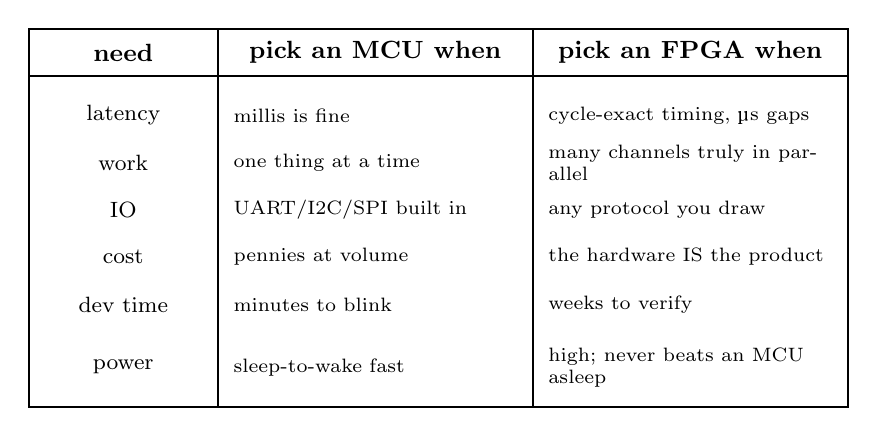
\begin{tikzpicture}[font=\scriptsize, >=latex]
% MCU vs FPGA decision table (deliverable figure)
\draw[thick] (0.2,0.2) rectangle (10.6,5.0);
\draw[thick] (0.2,4.4) -- (10.6,4.4);
\draw[thick] (2.6,0.2) -- (2.6,5.0);
\draw[thick] (6.6,0.2) -- (6.6,5.0);
\node[font=\small\bfseries] at (1.4,4.7) {need};
\node[font=\small\bfseries] at (4.6,4.7) {pick an MCU when};
\node[font=\small\bfseries] at (8.6,4.7) {pick an FPGA when};
\foreach \y/\l/\m/\f in {
  3.9/{latency}/{millis is fine}/{cycle-exact timing, \textmu s gaps},
  3.3/{work}/{one thing at a time}/{many channels truly in parallel},
  2.7/{I\/O}/{UART/I2C/SPI built in}/{any protocol you draw},
  2.1/{cost}/{pennies at volume}/{the hardware IS the product},
  1.5/{dev time}/{minutes to blink}/{weeks to verify},
  0.7/{power}/{sleep-to-wake fast}/{high; never beats an MCU asleep}}{
  \node[font=\footnotesize] at (1.4,\y) {\l};
  \node[align=left, text width=3.6cm] at (4.6,\y) {\m};
  \node[align=left, text width=3.6cm] at (8.6,\y) {\f};
}
\end{tikzpicture}
